
% This LaTeX was auto-generated from an M-file by MATLAB.
% To make changes, update the M-file and republish this document.

\documentclass{article}
\usepackage{graphicx}
\usepackage{color}
\usepackage{listings}
\usepackage[framed]{mcode}
\usepackage{fullpage}
\usepackage{hyperref}
\usepackage{amsmath}

\definecolor{lightgray}{gray}{0.5}
\setlength{\parindent}{0pt}

\begin{document}

    
    \begin{par}

\title{BE 521 - Homework 5\\{\normalsize Spring 2015}}
\author{Mike Lautman}
\date{\today}
\maketitle
\textbf{Objective:} Visual responses and likelihood.

\end{par}
\begin{lstlisting}
clf; close all; clear all; clc;
load mouseV1.mat
sec = 2;
\end{lstlisting}
\begin{par}

\section*{1 Stimulus Response}

\end{par}
\begin{par}

\subsection*{1.1 Unique grating angles}

\end{par}
\begin{lstlisting}
angle_cnt = length(unique(stimuli(:,2)))
\end{lstlisting}

\color{lightgray} \begin{lstlisting}
angle_cnt =

    12

\end{lstlisting} \color{black}
\begin{par}

\subsection*{1.2 Tuning Curve}

\end{par}
\begin{lstlisting}
neuron_cnt = length(neurons);
fire_cnt = zeros(neuron_cnt, angle_cnt);
angle_stim_cnt = zeros(1, angle_cnt);
stimuli_angles = sort(unique(stimuli(:,2)));
for i=1:length(stimuli)
    ts = stimuli(i,1);
    angle = stimuli(i,2);
    angle_i = angle/30 + 1;
    angle_stim_cnt(angle_i) = angle_stim_cnt(angle_i) + 1;
    for j = 1:neuron_cnt
        if find(ts < neurons{j} & ts + sec * 1000 > neurons{j})
            fire_cnt(j, angle_i) = fire_cnt(j, angle_i) + 1;
        end
    end
end

fire_ave = bsxfun(@rdivide, fire_cnt, angle_stim_cnt);


figure(1)
hold on
for i=1:4
    subplot(2,2,i)
    plot(stimuli_angles, fire_ave(i,:));
    title(strcat('Tuning Curve for Neuron #', num2str(i)))
    xlabel('Stimulus Angle (Degrees)');
    ylabel('Spikes (Cnt)')
    xlim([0 360])
    ylim([0 1])
end
\end{lstlisting}


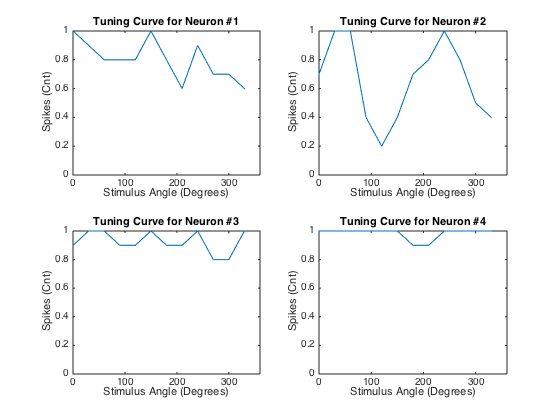
\includegraphics [width=4in]{mlautman_hw5_01.png}
\begin{par}

\subsection*{1.2.a}
It is reasonable to assume that the respone of a cell to stimulus at
$\theta$ will be equal to $\theta + 180$ since the images at these angles
will be equivalent. In practice however, the experimnetal data is very
noisy. We show this by plotting 9 neuron's tuning curves alongside
their tuning curves shifted by $180$ degrees. Some neurons exibit the
expected behavior while others do not.

\end{par}
\begin{lstlisting}
figure(2)
hold on
for i=1:4
    subplot(2,2,i)
    hold on
    plot(stimuli_angles, fire_ave(i,:), 'b');
    plot(stimuli_angles, [fire_ave(i,7:12), fire_ave(i,1:6)]-.005, 'r');
    title(strcat('TC for Neuron #', num2str(i)))
    xlabel('Stimulus Angle (Degrees)');
    ylabel('Spikes (Cnt)')
    legend('base', 'shifted','Location','best')
    xlim([0 360])
    ylim([0 1])
end
\end{lstlisting}


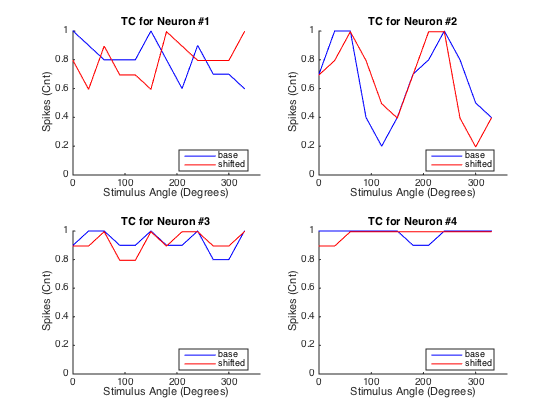
\includegraphics [width=4in]{mlautman_hw5_02.png}
\begin{par}

\subsection*{1.2.b}
Given what we know about cells in V1 this has physiological justification.
Since the neurons themselves act much like gabor transforms.

\end{par}
\begin{par}

\section*{2 Neural Decoding}

\end{par}
\begin{par}

\subsection*{2.1 Training}

\end{par}
\begin{lstlisting}
fire_cnt_bayes = zeros(neuron_cnt, angle_cnt/2);
angle_stim_cnt_bayes = zeros(1, angle_cnt/2);
for i=1:70
    ts = stimuli(i,1);
    angle = stimuli(i,2);
    angle = mod(angle, 180);
    angle_i = angle/30 + 1;
    angle_stim_cnt_bayes(angle_i) = angle_stim_cnt_bayes(angle_i) + 1;
    for j = 1:neuron_cnt
        if find(ts < neurons{j} & ts + sec * 1000 > neurons{j})
            fire_cnt_bayes(j, angle_i) = fire_cnt_bayes(j, angle_i) + 1;
        end
    end
end
fire_ave_bayes = bsxfun(@rdivide, fire_cnt_bayes, angle_stim_cnt_bayes);

figure(3)
hold on
edges = 0:30:360;
histogram(stimuli(1:70,2),edges)
title('Stimulus Angle Counts')
ylim([0, 10])
xlim([0,360])
xlabel('Stimulus angle (Degrees)')
ylabel('Count')
\end{lstlisting}


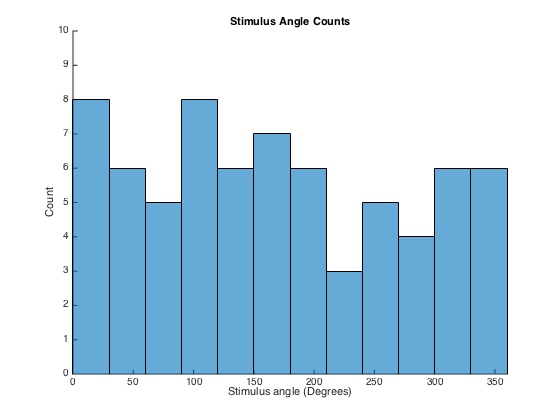
\includegraphics [width=4in]{mlautman_hw5_03.png}
\begin{par}

\subsection*{2.2 Testing}

\end{par}
\begin{lstlisting}
S = zeros(neuron_cnt, 50);
test_c = zeros(50,1);
for i=1:50
    k = i + 70;
    ts = stimuli(k,1);
    angle = stimuli(i,2);
    angle = mod(angle, 180);
    test_c(i) = angle;
    for j = 1:neuron_cnt
        if find(ts < neurons{j} & ts + sec * 1000 > neurons{j})
            S(j, i) = S(j, i) + 1;
        end
    end
end
fire_ave_bayes_pad = fire_ave_bayes + (fire_ave_bayes==0)*.0001;
L_test = S'*log(fire_ave_bayes_pad);
\end{lstlisting}
\begin{par}

\subsection*{2.2.a }

\end{par}
\begin{lstlisting}
figure(4)
hold on
for i=1:4
    subplot(2,2,i)
    plot(stimuli_angles(1:6), L_test(i,:))
    t = sprintf('Likelihood angle test #%d, (Actual Ang %d)',i, test_c(i));
    title(t)
    xlabel('Stimulus Angle (Degrees)');
    ylabel('Class prediction')
    xlim([0, 180])
end
\end{lstlisting}


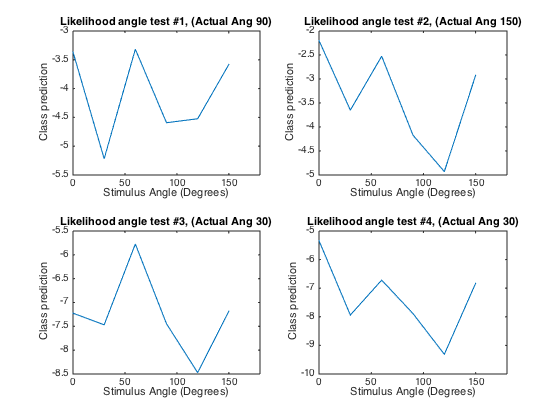
\includegraphics [width=4in]{mlautman_hw5_04.png}
\begin{par}

\subsection*{2.2.b}
These four likelihood functions do not seem to match the true simulation
angle well at all. This is likely a result of noisy data with
insufficient sample size to overcome the noise. Furthermore, the number
of featues is very low, further complicating the issue.

\end{par}
\begin{par}

\subsection*{2.2.c MLE}

\end{par}
\begin{lstlisting}
[~,MLE] = max(L_test,[],2);
MLE = (MLE-1) * 30;
accuracy = mean(test_c == MLE)
\end{lstlisting}

\color{lightgray} \begin{lstlisting}
accuracy =

    0.1800

\end{lstlisting} \color{black}
\begin{par}

\subsection*{2.2.d Accuracy issues}
The accuracy of this method is only slightly better than guessing. To
Imporove this we should use much more training data and more features if
we can get them. We could also project the features into a higher
dimension using a kernel method to increase the complexity of the
decision surface which may also help.

\end{par}
\begin{par}

\subsection*{2.3.a Permutation Test}

\end{par}
\begin{lstlisting}
num_tests = 1000;
permutation_test = zeros(num_tests, 6);
pt = zeros(num_tests,1);
for i=1:num_tests
    test_c_p = (randi(7, [50,1]) - 1) * 30;
    for j=1:6
        permutation_test(i,j) = ...
            sum((test_c_p == MLE) & (test_c_p == 90))/...
            sum(test_c_p == (j-1)*30);
    end
    pt(i) = mean(test_c_p == MLE);
end

figure(5)
hold on
histogram(pt)
l = line([accuracy, accuracy], [0,180],'Color','r');
title('Permutation Test')
xlabel('Expected Random Accuracy (%)')
ylabel('Count (1000 total)')
legend(l, 'Experimental Accuracy','Location', 'best');
\end{lstlisting}


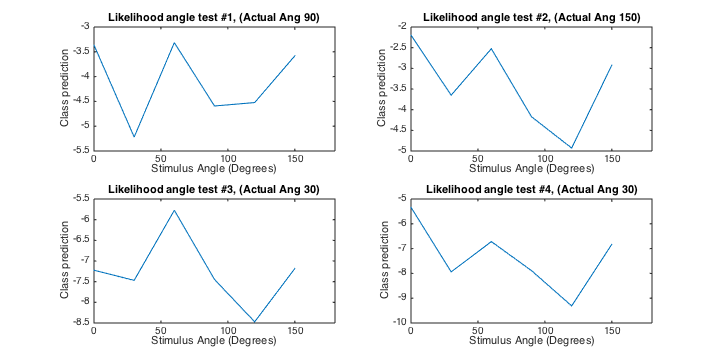
\includegraphics [width=4in]{mlautman_hw5_05.png}


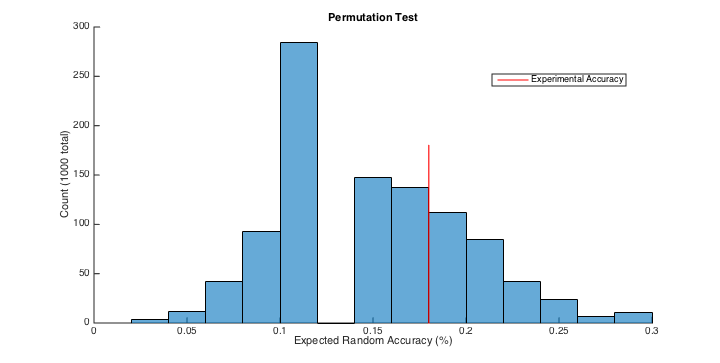
\includegraphics [width=4in]{mlautman_hw5_06.png}
\begin{par}

\subsection*{2.3.b}

\end{par}
\begin{lstlisting}
if accuracy > mean(pt)
    frac = mean(pt > accuracy)
else
    frac = mean(pt < accuracy)
end
\end{lstlisting}

\color{lightgray} \begin{lstlisting}
frac =

    0.1690

\end{lstlisting} \color{black}
\begin{par}

\subsection*{2.4}
This is truly an error in experimental design. What the experimenters
should have used is called Term Frequency Inverse Document frequency or
TF-IDF. This method would deal with the issue of 'swamping' the log
likelihood estimates because any neuron that simply likes to fire a lot
would be given less weight per firing. The calculation of this is fairly
simple. We would count up the neuron firings for each angle and divide by
the angle frequency creating an $18x6$ matrix $F$ as we did before, but
we would also divide each row by the row totals, thus normalizing the
influence of each neuron.

\end{par}
\begin{lstlisting}
clf; clear all; close all;
\end{lstlisting}



\end{document}
    
